% compile with XeLaTeX
% this template was created by salim bou 
\documentclass[dvipsnames,mathserif]{beamer}
\mode<presentation>
\usepackage{tikz}
\usetikzlibrary{calc}
\usepackage{listings}
\usepackage{xcolor}
\usepackage{mathtools}
 \usepackage[LAE,T1]{fontenc}
%\usepackage[arabic,french,english]{babel}
 
\usepackage{verbatim}

\usetikzlibrary{arrows,shapes,backgrounds}

 \newcommand{\rtx}[1]{\textcolor{red}{#1}}
 
\newcommand{\fr}{\selectlanguage{french}}
 
\newcommand{\gfcb}[1]{%
    \fcolorbox{white}{gray!10!}{\quad\strut #1\quad}
    } % gfcb := gray fcolorbox
\newcommand{\cop}[1]{%
    \ensuremath{\quad\longrightarrow\quad #1}
    \gfcb{\texttt{\detokenize{#1}}} 
    %\ensuremath{\quad\longrightarrow\quad #1}
    } % cop := code output

\usepackage{hyperref}
\newcommand*{\email}[1]{%
    \normalsize\href{mailto:#1}{#1}\par
}
\usepackage{polyglossia}
\setdefaultlanguage[numerals=maghrib,locale=algeria]{arabic} % locale=mashriq, libya, algeria, tunisia, morocco, or mauritania  for names of months in \date 
\setotherlanguage{english}
\newfontfamily\arabicfont[Script=Arabic]{Lateef}
\newfontfamily\arabicfontsf[Script=Arabic]{Lateef}

%\usetheme{Madrid}
\usetheme{modprogressbarMAHER}
%\usecolortheme{crane}
\usetikzlibrary{fadings, backgrounds}
\tikzfading[name=fade out, inner color=transparent!100, outer color=transparent!40]
\tikzfading[name=fade in, inner color=transparent!100, outer color=transparent!0]
%\usetikzlibrary{mindmap}
\usetikzlibrary{shadows}
\usetikzlibrary{shapes,arrows,positioning,automata,backgrounds,calc,er,patterns}

\usepackage{tikz-feynman}

\tikzfeynmanset{compat=1.0.0}
\usetikzlibrary{decorations.pathmorphing, patterns,shapes}

\usepackage[beamer]{hf-tikz}
 
\usetikzlibrary{overlay-beamer-styles}
\tikzset{
	highlight on/.style={alt={#1{fill=red!80!black,color=red!80!black}{fill=gray!30!white,color=gray!30!white}}},
}

%\tikzset{
%	basic/.style  = {draw, text width=2cm, drop shadow, font=\sffamily, rectangle},
%	root/.style   = {basic, thin, align=center,
%		fill=gray!45},
%	level 2/.style = {basic, thin,align=center, fill=gray!30,
%		text width=8em},
%	level 3/.style = {basic, thin, align=left, fill=gray!20, text width=6.5em}
%}
 \tikzset{
 	basic/.style  = {draw, text width=4cm, drop shadow, font=\sffamily, rectangle},
 	root/.style   = {basic, rounded corners=2pt, thin, align=center,
 		fill=green!30},
 	level 2/.style = {basic, rounded corners=3pt, thin,align=center, fill=green!60,
 		text width=10em},
 	level 3/.style = {basic, thin, align=left, fill=pink!60, text width=7.8em}
 }
 
\tikzset{
	pivot/.style={
		draw, 
		regular polygon, 
		regular polygon sides = 3, 
		fill = red, 
		node distance = 1cm, 
		minimum height = 2em,
		at = {(0,0)}
	}
}
% for RTL liste
\makeatletter
\newcommand{\RTListe}{\raggedleft\rightskip\leftm}
\newcommand{\leftm}{\@totalleftmargin}
\makeatother



% RTL frame title
\setbeamertemplate{frametitle}
{\vspace*{-1mm}
  \nointerlineskip
    \begin{beamercolorbox}[sep=0.3cm,ht=2.2em,wd=\paperwidth]{frametitle}
        \vbox{}\vskip-2ex%
        \strut\hskip1ex\insertframetitle\strut
        \vskip-0.8ex%
    \end{beamercolorbox}
}


% align subsection in toc
\makeatletter
\setbeamertemplate{subsection in toc}
{\leavevmode\rightskip=5ex%
  \llap{\raise0.1ex\beamer@usesphere{subsection number projected}{bigsphere}\kern1ex}%
  \inserttocsubsection\par%
}
\makeatother

% RTL triangle for itemize
\setbeamertemplate{itemize item}{\scriptsize\raise1.25pt\hbox{\donotcoloroutermaths$\blacktriangleleft$}} 

%\setbeamertemplate{itemize item}{\rule{4pt}{4pt}}

\defbeamertemplate{enumerate item}{square2}
{\LR{
    %
    \hbox{%
    \usebeamerfont*{item projected}%
    \usebeamercolor[bg]{item projected}%
    \vrule width2.25ex height1.85ex depth.4ex%
    \hskip-2.25ex%
    \hbox to2.25ex{%
      \hfil%
      {\color{fg}\insertenumlabel}%
      \hfil}%
  }%
}}

\setbeamertemplate{enumerate item}[square2]

\setbeamertemplate{navigation symbols}{}

%%%%%%%%%%%%%%%%%%%%%%%%%%%%[ blocks ]%%%%%%%%%%%%%%%%%%%%%%%%%%%%%%%%%%%%
\newenvironment<>{problock}[1]{%
	\begin{actionenv}#2%
		\def\insertblocktitle{#1}%
		\par%
		\mode<presentation>{%
			%\setbeamercolor{block title}{fg=white,bg=blue!48!black}
			\setbeamercolor{block body}{fg=white,bg=pbblue}
			%  \setbeamercolor{itemize item}{fg=orange!20!black}
			%  \setbeamertemplate{itemize item}[triangle]
		}%
		\usebeamertemplate{block begin}}
	{\par\usebeamertemplate{block end}\end{actionenv}}
 
%=========================================================================
\begin{document}
 

%\title{ تعلم LaTeX في 60 دقيقة}
\title{كورس مكثف لتعلم الLaTeX على محرر Overleaf}
\logo{
\includegraphics[width=0.5cm]{figs/sudan_logo.png}}
\author[Mohammed M. A. Mohammed]{ \href{https://www.facebook.com/mohammedmaher8932/}{\it{محمد ماهر عبد الرحيم محمد}}  }
\institute{\href{https://www.facebook.com/groups/651884204836245}{\Large{ملتقى الفيزيائيين السودانيين}} 
 
}
\vspace{-2cm}
%\date{\today}
%\affil{\it{The Insider Researcher Group, Khartoum, Sudan}\\

\date{10/02/2023}
\begin{frame}

\begin{center}
\maketitle

\includegraphics[scale=0.1]{figs/sfp.jpg}
    
\includegraphics[scale=0.2]{figs/online-editor-2.png}
    
\includegraphics[scale=0.1]{figs/sfp.jpg}
    
\end{center}

\end{frame}

%=============================================================================
\begin{frame}{التعريف ببرنامج الدورة}
\begin{itemize}\RTListe
 \item
اليوم الأول: مدخل إلى \LaTeX{}
\begin{itemize}\RTListe
   \item
    مقدمة عن \LaTeX{} واستخداماته
     
       \item
    هيكل الوثيقة الأساسية وتنسيقها
      \item
    إنشاء أقسام وفقرات وفواصل أسطر
    \item
    التنسيق الرياضي الأساسي
\end{itemize}
\item
اليوم الثاني: تنسيق \LaTeX{} المتقدم
\begin{itemize}\RTListe
   \item
    عمل الجداول والأشكال
   \item
    استخدام حزم \LaTeX{}
       \item
    تنسيق رياضي متقدم
    إنشاء الببليوجرافيات والاستشهادات
       \item
    إنشاء وحدات ماكرو وبيئات مخصصة
\end{itemize}
\item
اليوم الثالث: أفضل الممارسات والتطبيقات
\begin{itemize}\RTListe
   \item
    أفضل الممارسات لتصميم مستندات \LaTeX{}
     \item
    التعاون في مشاريع \LaTeX{}
      \item
    إنشاء عروض تقديمية باستخدام \LaTeX{}
      \item
    إنشاء المقالات والتقارير العلمية باستخدام \LaTeX{}
    تكامل \LaTeX{} مع الأدوات والتقنيات الأخرى
\end{itemize}
\end{itemize}
\end{frame}
%==========================================================
%////////////////////////////////////////////////////////////////////////////////////
%===================================================================================
\begin{frame}[plain]
	\addtocounter{framenumber}{-1}
	\begin{problock}{}
		\LARGE
		\vfill
		\centerline{\bf \textcolor{white}{\bf اليوم الأول: الأساسيات}}		
		\vfill
	\end{problock}
 
\end{frame}
%==========================================================
\begin{frame}{المحتويات}
\tableofcontents
\end{frame}
%=========================================================
\section{ما هو \LaTeX\ ولماذ نحتاجه  }

\begin{frame}{ما هو \LaTeX\ ولماذ نحتاجه  }
\begin{exampleblock}{\LaTeX{}}
 
هو نظام إعداد الوثائق و المستندات يستخدم في كتابة (االأوراق العلمية، البحوث، التقارير و الكتب ...) عالية الجودة بدقة واتساق كبيرين
\end{exampleblock}
 \begin{center}
   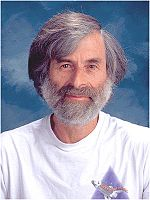
\includegraphics[scale=0.35]{figs/Lamport.png} 
     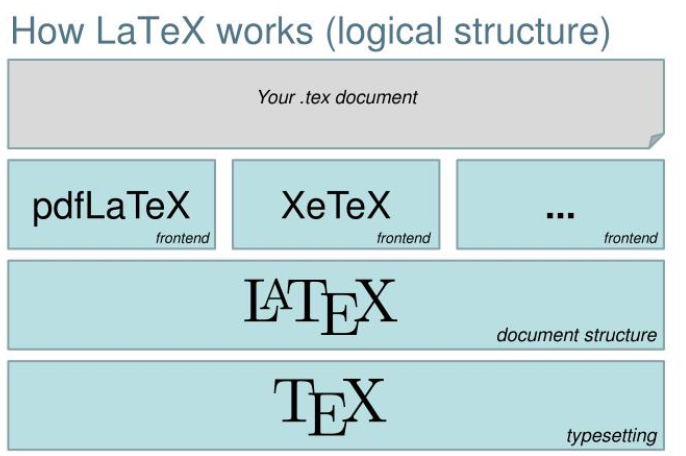
\includegraphics[scale=0.25]{figs/howLW.png}
   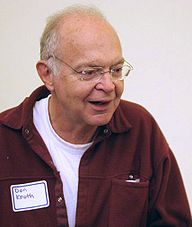
\includegraphics[scale=0.35]{figs/knuth.png} 
 \end{center}
 
\end{frame}
%==============================================
\begin{frame}[shrink=15]\frametitle{المميزات}
 
المميزات:
\begin{itemize}\RTListe
    \item يوفر التحكم الكامل في التنسيق الصفحة، مما يجعل النصوص الأكاديمية والعلمية جيدة الشكل ولطيفة المشاهدة.
    \item يجعل العمل مع الجداول والصور و الفقرات النصية سهلاً ويسهل التنسيق الجانبي.
    \item يوفر الدعم الكامل لللغات بما فيهم العربية.
    \item يجعل التعامل مع الإشارات المرجعية الأكاديمية والأعداد الإحصائية و الجداول سهلاً.
    \item يعطي الملف في شكل PDF او PS جاهزة للطباعة  .
\end{itemize}

 \begin{center}
     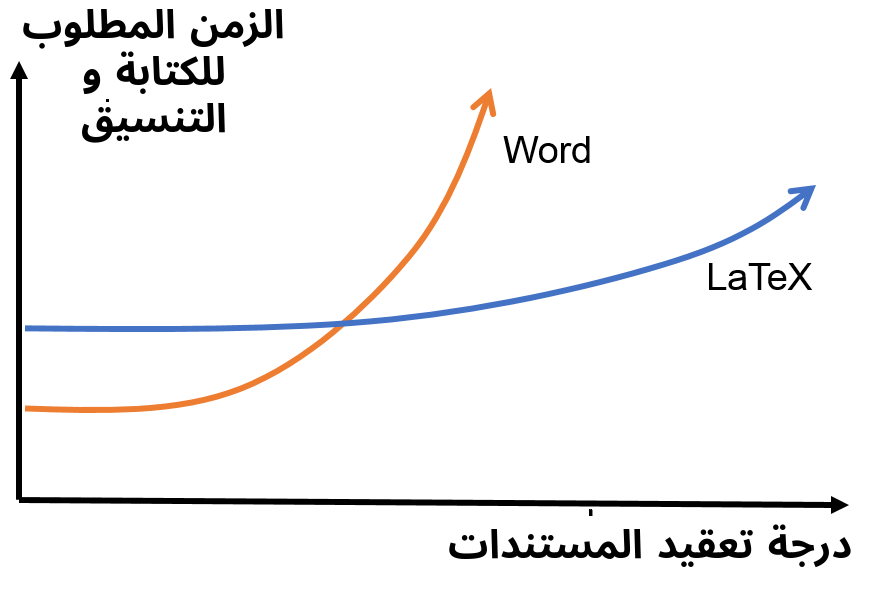
\includegraphics[scale=0.25]{figs/word_vs_latex_1_eng.png}
 \end{center}
 
\end{frame}
%==============================================
\begin{frame}{محررات نصوص ال\LaTeX{}}
    \begin{itemize}\RTListe
        \item 
    \href{https://miktex.org/download}{\textcolor{blue}{MiKTeX}} لنظام التشغيل Windows
    \item
   \href{https://www.tug.org/texlive/}{\textcolor{blue}{TeX Live}} لنظام التشغيل Linux والأنظمة الأخرى المشابهة لـ UNIX
    \item
    إعادة توزيع \href{https://www.tug.org/mactex/}{\textcolor{blue}{MacTeX}} لـ TeX Live لنظام التشغيل macOS
    \item
    \href{https://www.tug.org/tetex/}{\textcolor{blue}{teTeX}} لنظام التشغيل Linux والأنظمة الأخرى المشابهة لـ UNIX ؛ لم يعد يتم صيانته بنشاط الآن
    يعتمد proTeXt على MiKTeX
    \end{itemize}
\begin{center}
    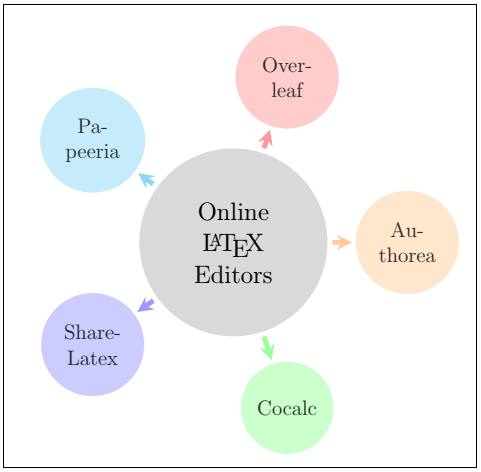
\includegraphics[width=5cm]{figs/latex-online-editors.png}
\end{center}
 %   \href{http://www.overleaf.com/}{\textcolor{green}{\bf http://www.overleaf.com/}}
\end{frame}
%==============================================
\begin{frame}[shrink=15]{منصة Overleaf}
\begin{itemize}\RTListe
    \item  \href{http://www.overleaf.com/}{\textcolor{green}{\bf :Overleaf}} محرر \LaTeX{} تعاوني يسمح للمستخدمين
لإنشاء وتحرير ومشاركة المستندات المكتوبة بلغة لاتك.
\end{itemize}
\begin{center}
    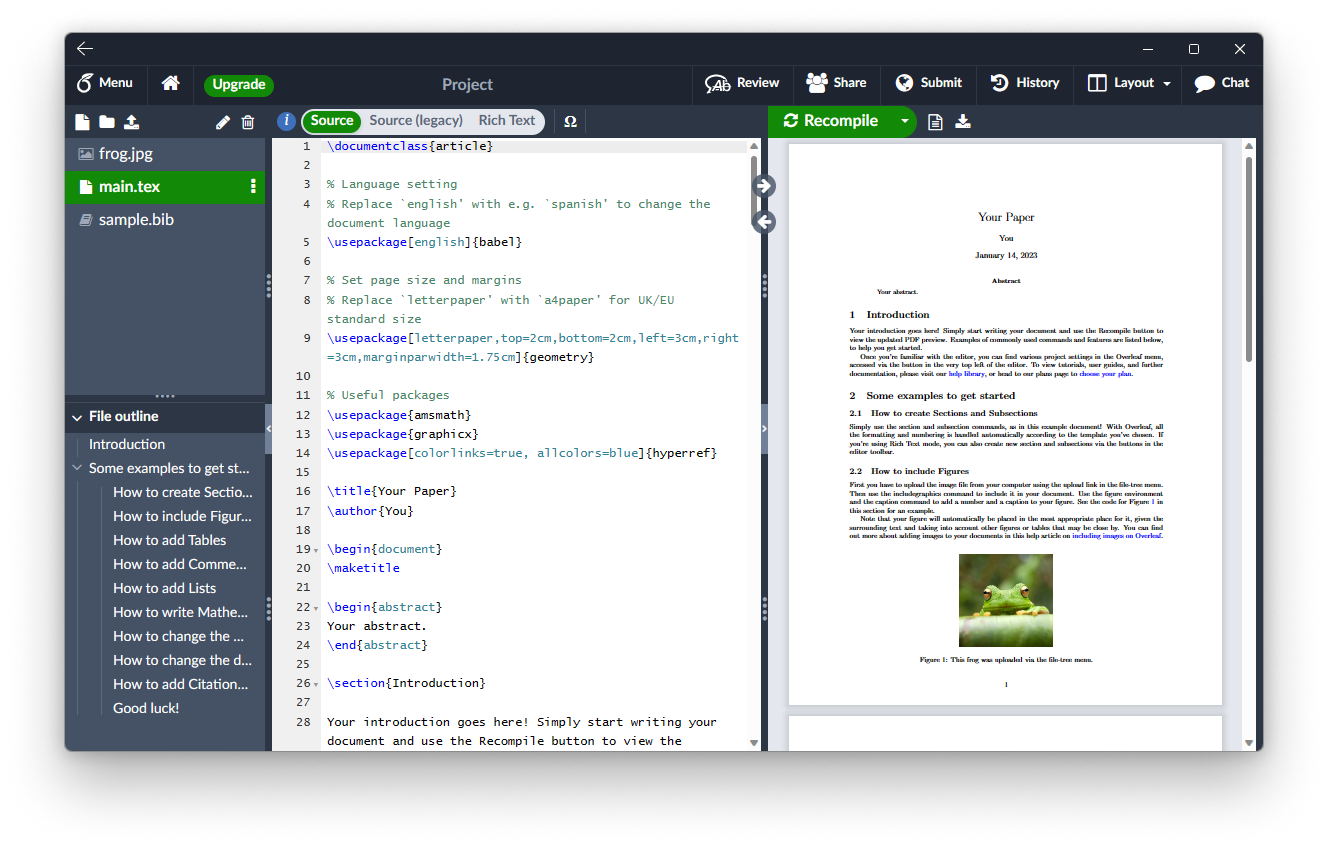
\includegraphics[scale=0.20]{figs/Screenshot_of_Overleaf.png}
\end{center}
\begin{itemize}\RTListe
    \item \textcolor{red}{محرر على الإنترنت}: دون الحاجة إلى تثبيت محلي لـ \LaTeX{}.
    \item
\textcolor{red}{التعاون}: من السهل على الفرق التعاون في مشروع ما.
\item
\textcolor{red}{القوالب}: من السهل على المستخدمين البدء بمشروع جديد.
\item
\textcolor{red}{التكامل مع الخدمات الأخرى}: مزامنة المستندات والوصول إليها من خدمات أخرى
المنصات.
\item
\textcolor{red}{المشاركة والنشر}: الإرسال المباشر.
\end{itemize}
    
\end{frame}
%==============================================
\section{قم بإنشاء مستندك الأول في  \LaTeX\ }
\begin{frame}[shrink=25]{قم بإنشاء مستندك الأول في  \LaTeX\ }
 %\begin{minipage}{0.495\textwidth}
 %\includegraphics[scale=0.20]{figs/example0.png}
% \end{minipage}
   % \centering
%\includegraphics[scale=0.2]{figs/exam0.png}
  \begin{columns}
		\column{0.5\textwidth}
%		 \begin{verbatim}
%			\documentclass[12pt, a4paper]{article}
%			
%			\begin{document}
%				
%			\end{document}
%		\end{verbatim}
		\begin{center}
			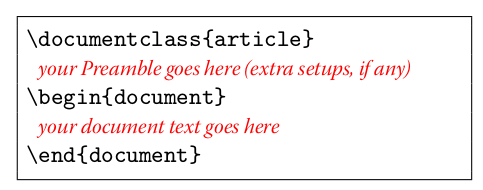
\includegraphics[scale=0.35]{figs/dstructure}
			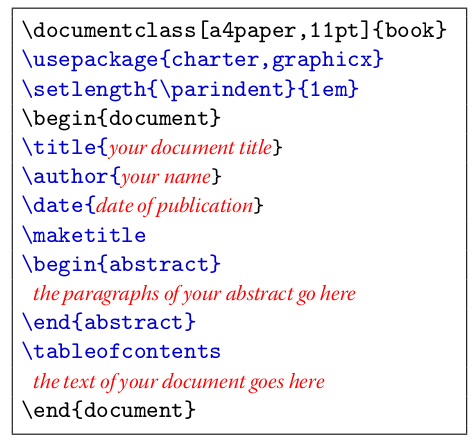
\includegraphics[scale=0.4]{figs/code1}
		\end{center}
	\column{0.5\textwidth}
		\begin{itemize}\RTListe
		
	  		\item الديباجة (Preamble) 
	  	
	  		\begin{itemize}\RTListe
	  			\item صَنْف المستند  class document \newline [ book.. report, article,  ]  
	  			\item حِزْمَ إضافية packages additional
	  		\end{itemize}
	  		
	  		\item مَتْن المستند body Document
	  \end{itemize}
   \bc
\includegraphics[scale=0.1]{autodraw 05_02_2023.png}\ec
	 		\underline{قواعد عامة}
 \begin{itemize}\RTListe
    \item[\checkmark]  تبدأ الاوامر بوضع شرطة مائلة للخلف($\backslash$) قبل كتابة اول حرف من الأمر
   \\
    علي سبيل \textcolor{green}{المثال}  \textcolor{green}{tableofcontents$\backslash$}
    \item[\checkmark] بعض الأوامر تحتاج إلى عَامِل لكي يظهر تأثيرها عليهايتم وضعها في اقواس معقوضة
   \\
    \textcolor{red}{مثال}:  \textcolor{red}{\{Ali\}}\textcolor{green}{author$\backslash$}
    \item[\checkmark] بعض الأوامر توفر خيارات إضافية، توضع هذه الخيارات بين اقواس مربعة
    \\
     \textcolor{red}{مثال}:   \textcolor{green}{\{book\}}\textcolor{red}{[a4paper,11pt]}\textcolor{green}{documentclass}\textcolor{green}{$\backslash$}.
\end{itemize}
	\end{columns}  
 
\end{frame}
%=============================================
\begin{frame}
 \bc
 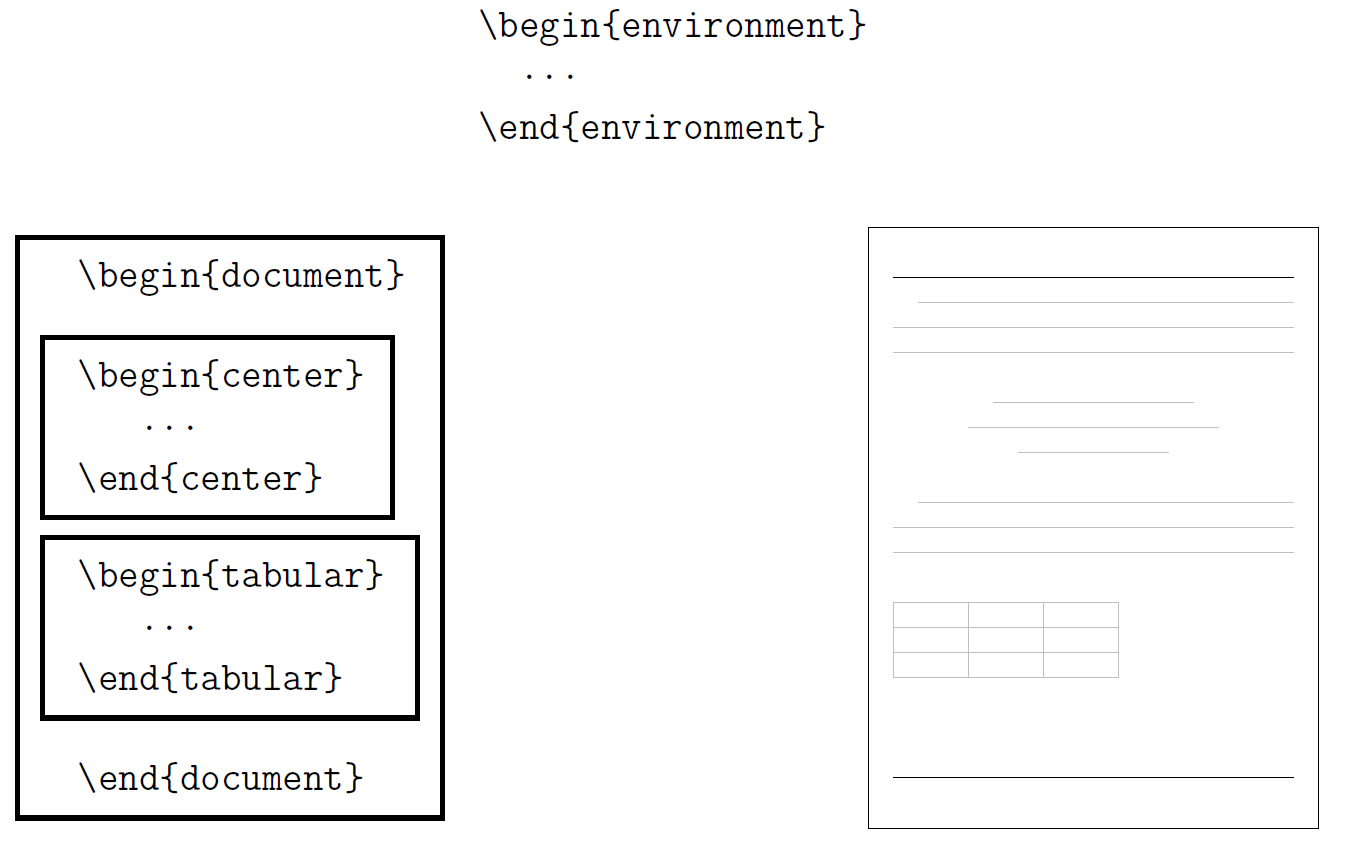
\includegraphics[scale=0.2]{figs/einv.png}
 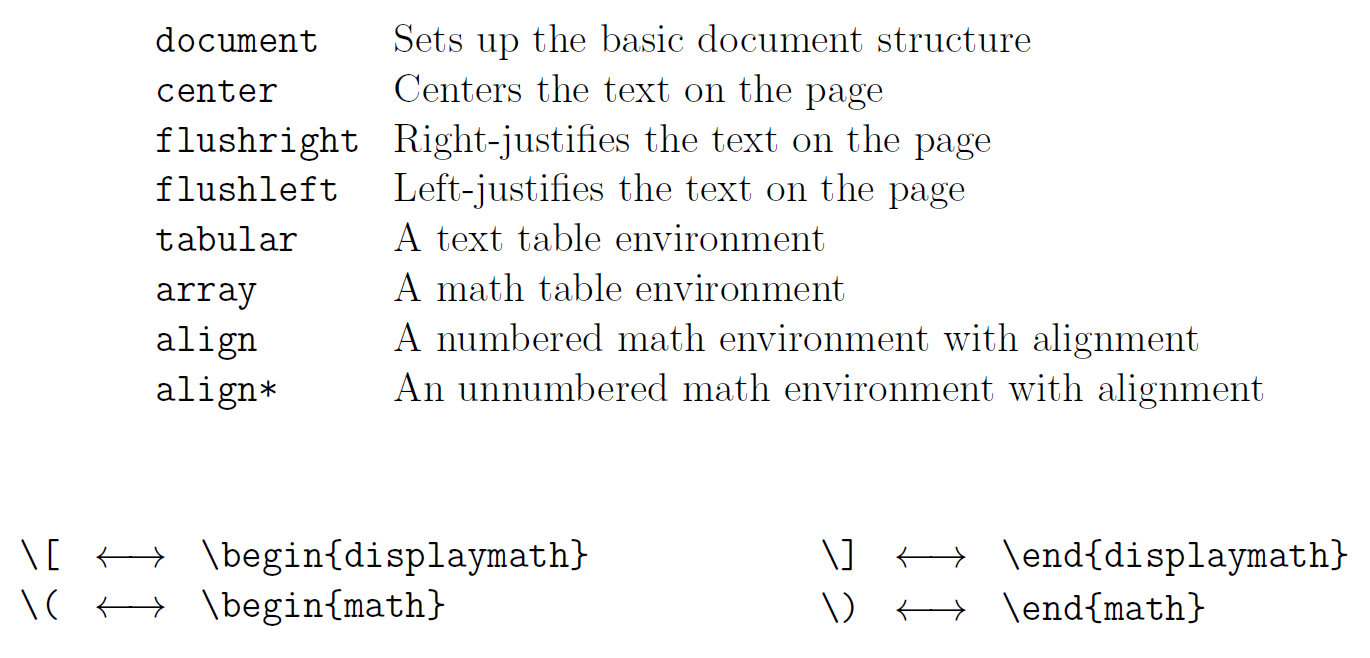
\includegraphics[scale=0.2]{figs/env2.png}
 \ec
 

\end{frame}
%==============================================
\begin{frame}
  \begin{columns}
		\column{0.5\textwidth}
		\begin{center}
			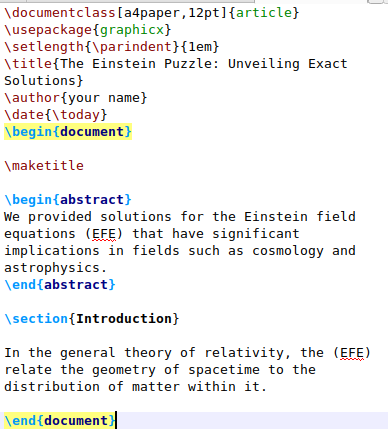
\includegraphics[scale=0.4]{figs/testo}
		\end{center}
	\column{0.5\textwidth}
 
	  \bc 
\includegraphics[scale=0.16]{figs/outtest} \ec
	\end{columns} 
\end{frame}
%==============================================
\section{فقرات وأسطر جديدة}
\begin{frame}{فقرات وأسطر جديدة}
\begin{center}
    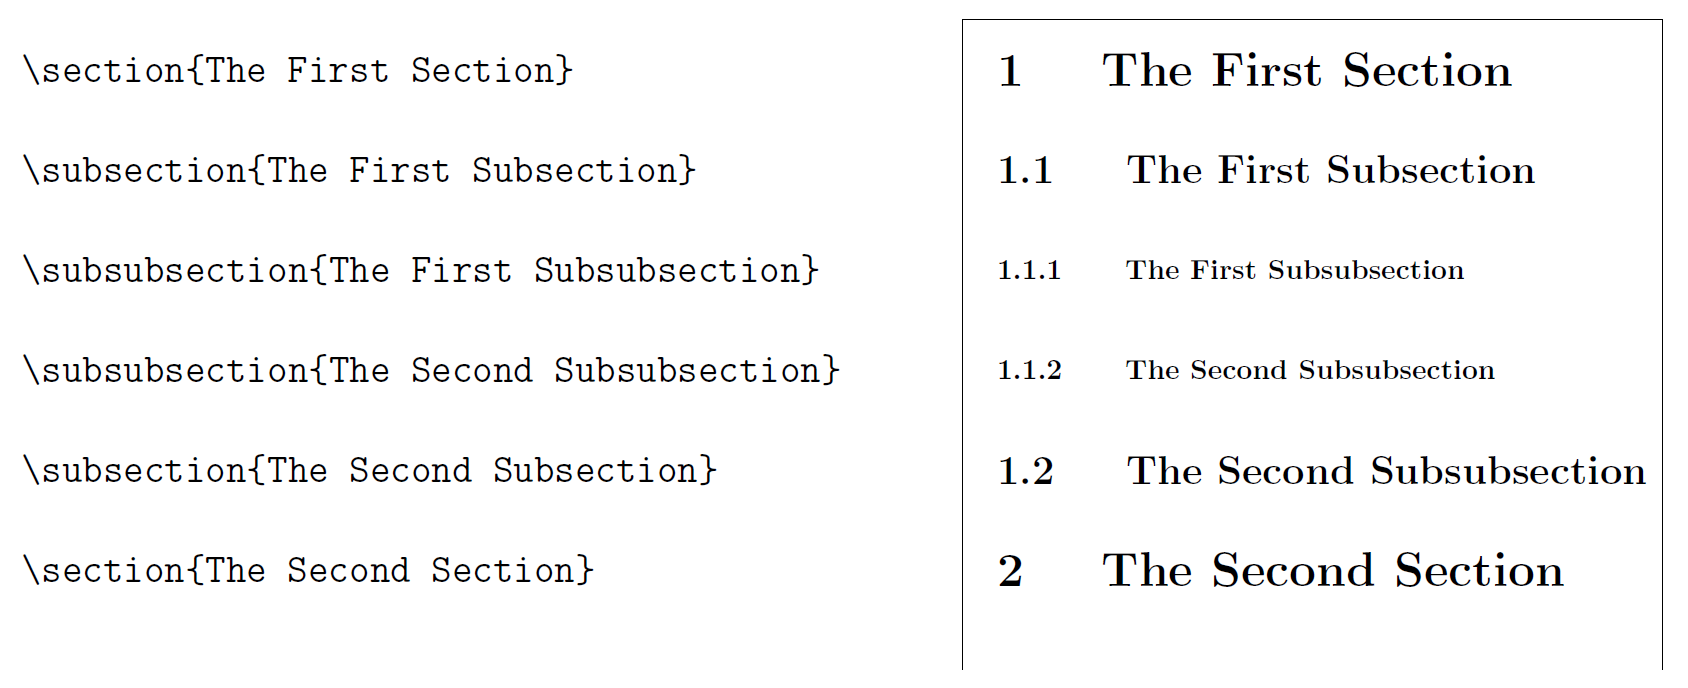
\includegraphics[width=11cm]{figs/sections.png}
\end{center}
\end{frame}
%==============================================
\begin{frame}{المحاذاة}
    \centering
    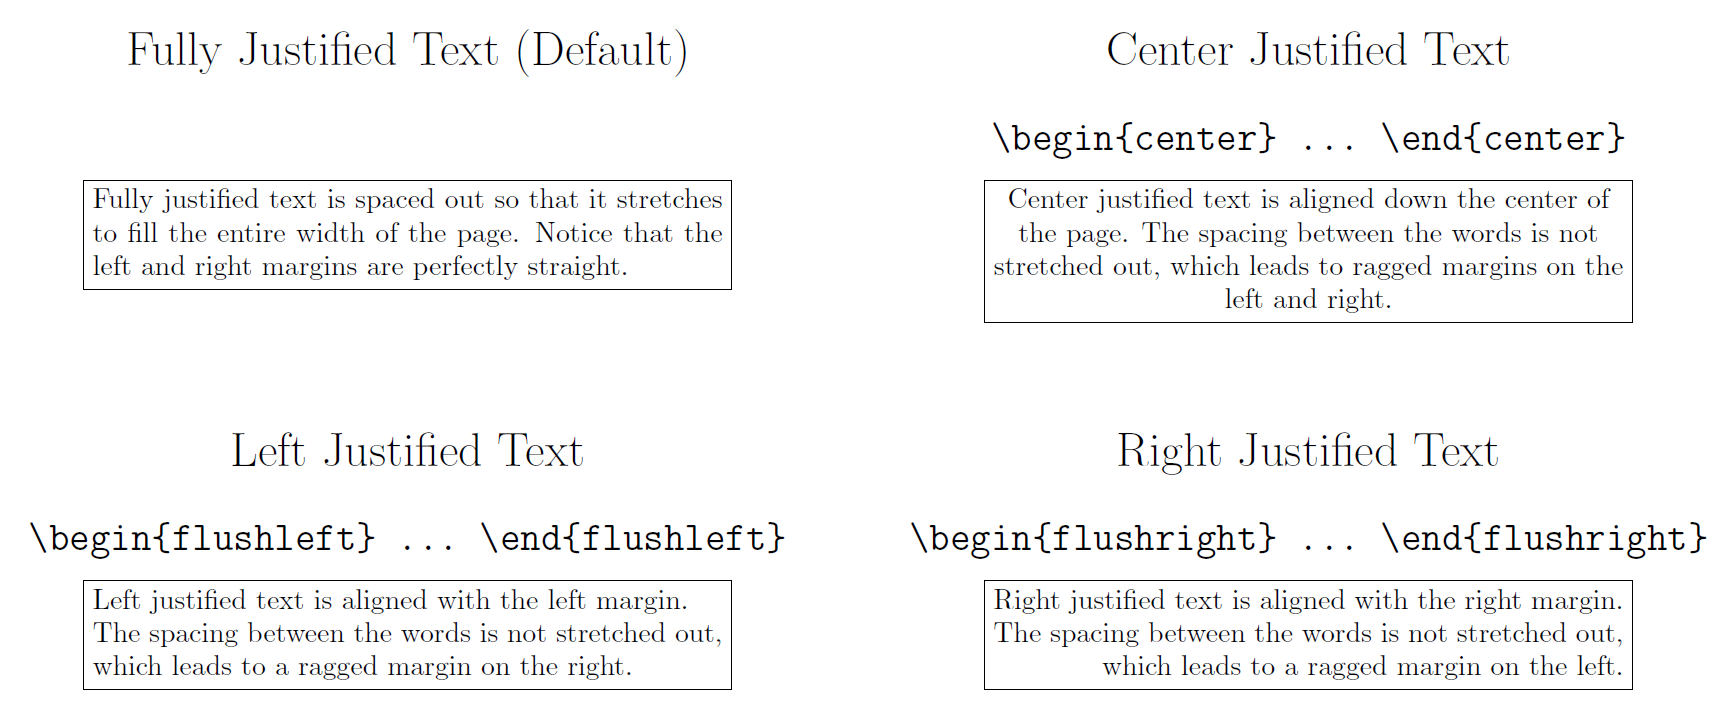
\includegraphics[width=11cm]{figs/paragraph1.png}
\end{frame}
%==============================================
\begin{frame}{الاسطر الجديدة}
    \centering
    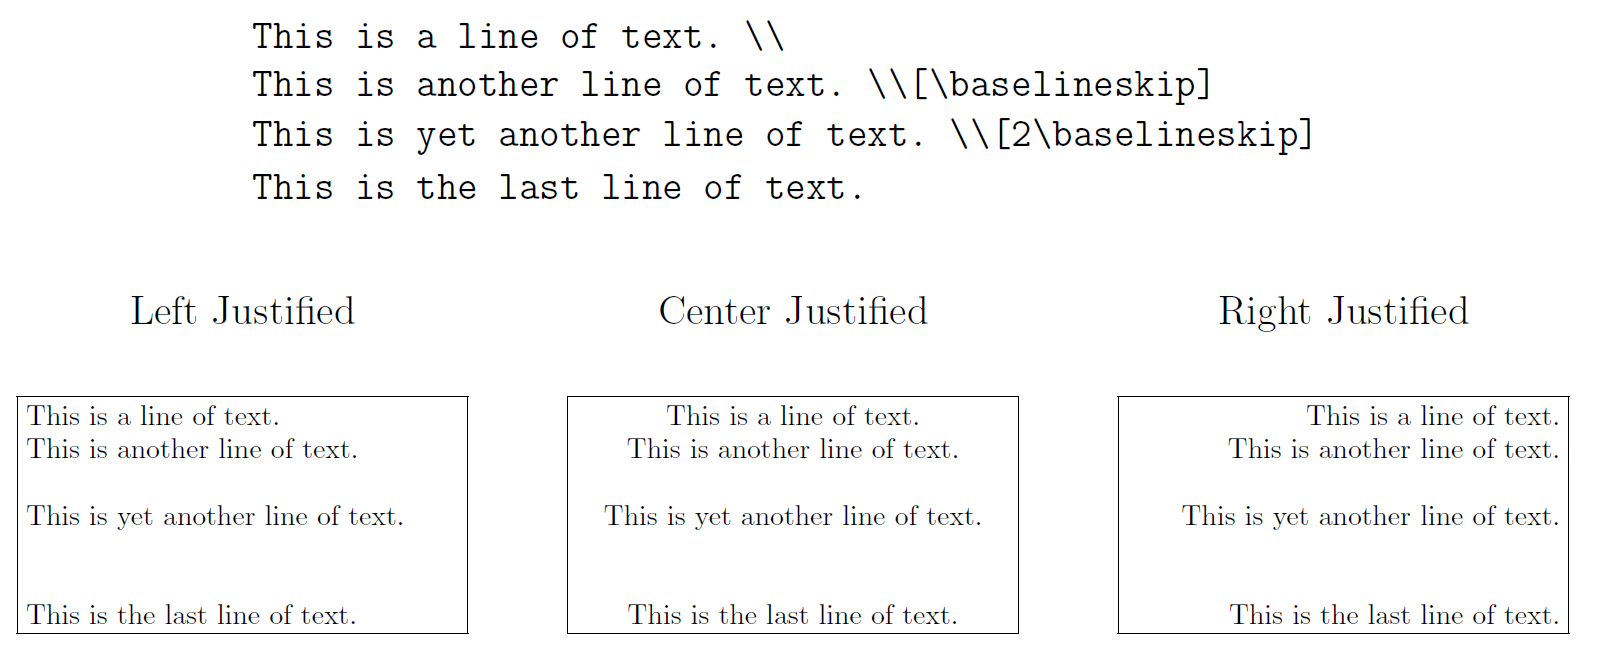
\includegraphics[width=11cm]{figs/paragraph2.png}
\end{frame}
%==============================================
\section{القوائم}
\begin{frame}{القوائم}
\begin{center}
    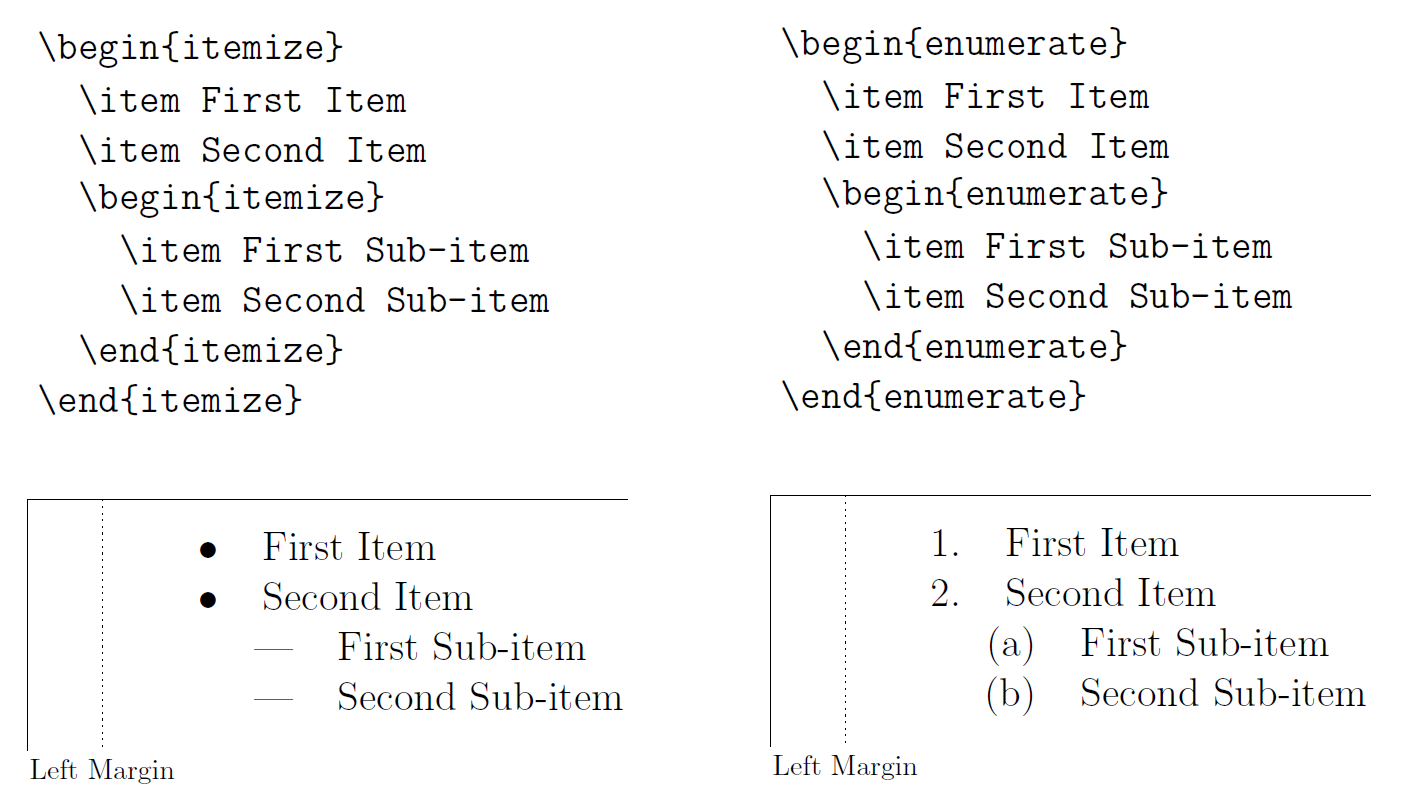
\includegraphics[scale=0.3]{figs/lists.png}
\end{center}
\end{frame}
%==============================================
\begin{frame}
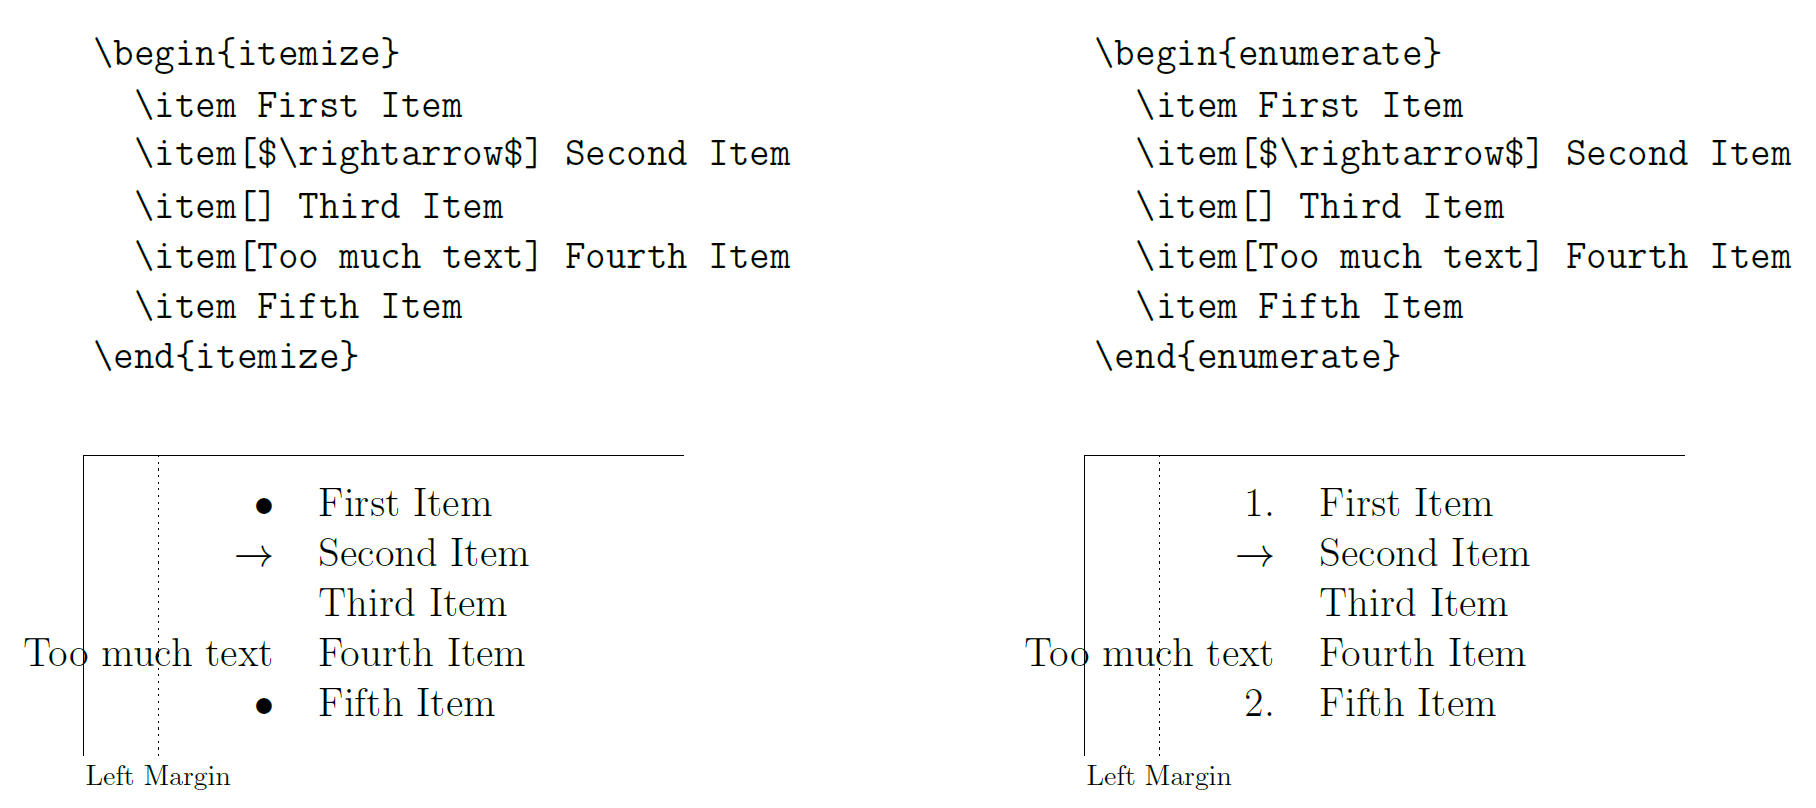
\includegraphics[width=11cm]{figs/lists2.png}
\end{frame}
%==============================================
\section{الصيغ الرياضية و الرموز}
\begin{frame}{الصيغ الرياضية و الرموز}
\begin{center}
    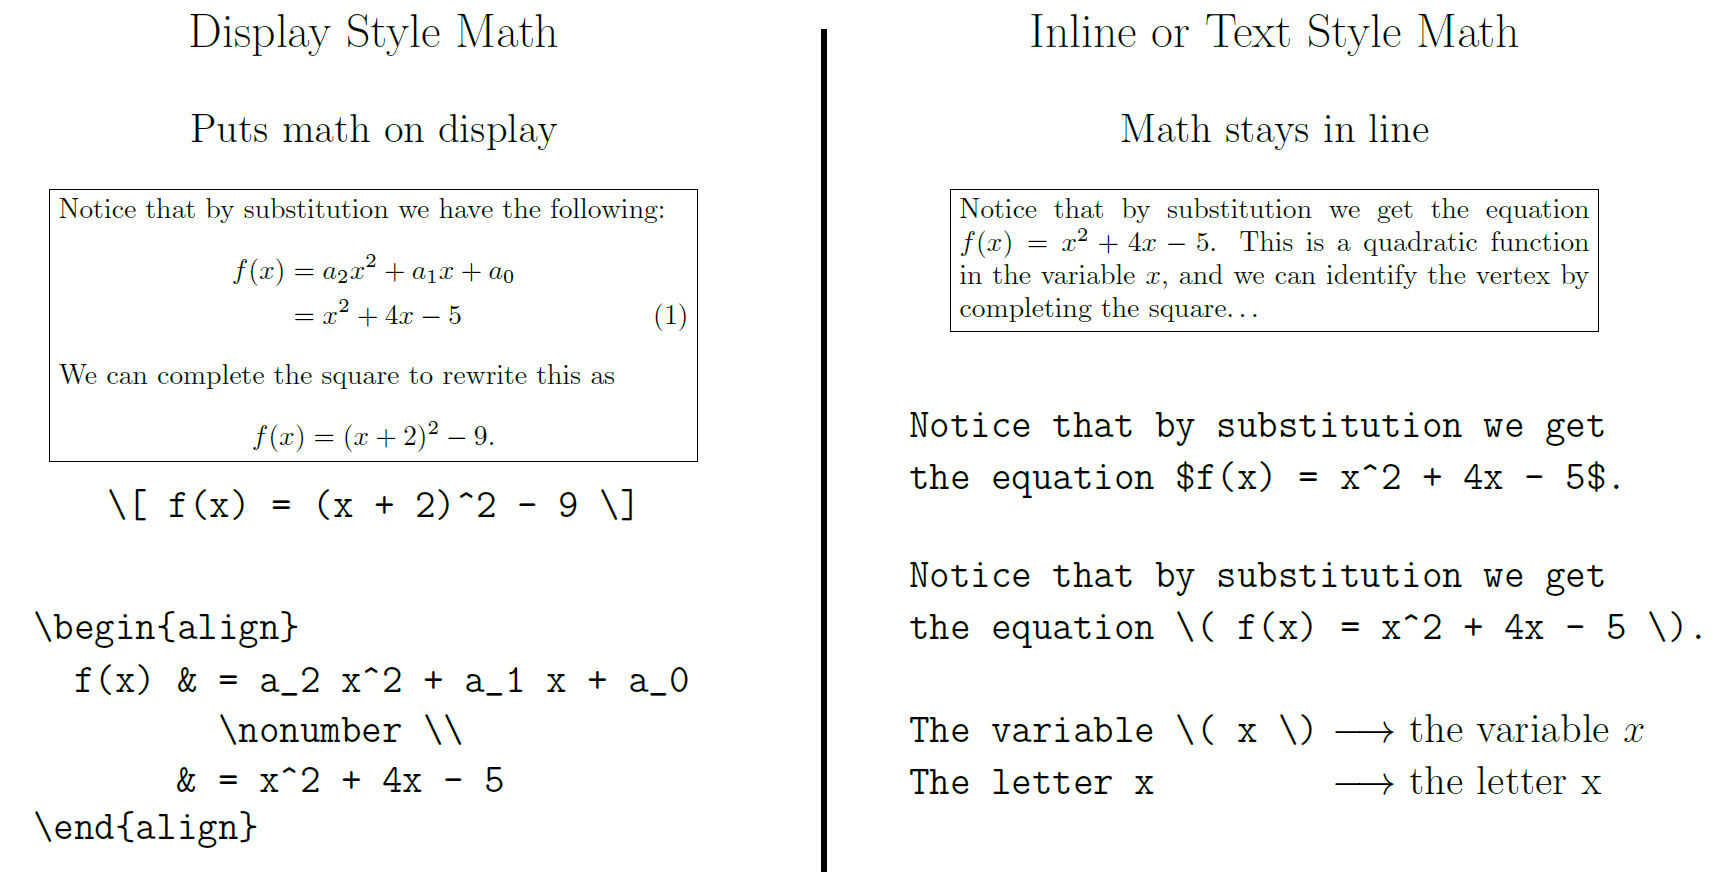
\includegraphics[width=11.5cm]{figs/math1.png}
\end{center}
\end{frame}
%==============================================
\begin{frame}{الصيغ الرياضية و الرموز}
\begin{center}
    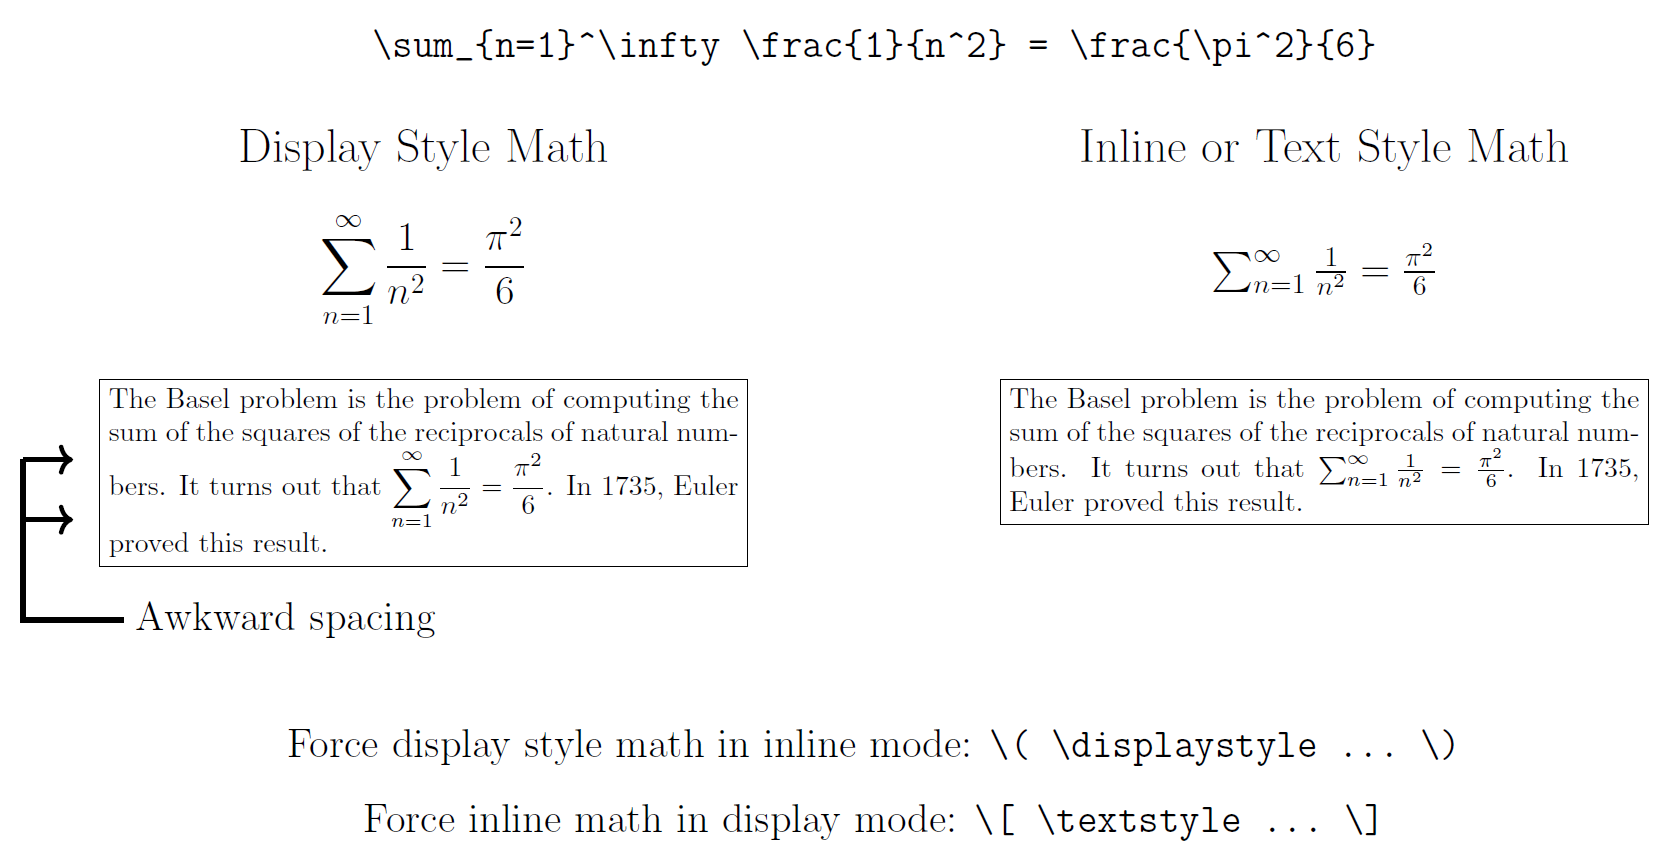
\includegraphics[width=11.5cm]{figs/math2.png}
\end{center}
\end{frame}
%==============================================
\begin{frame}{الصيغ الرياضية و الرموز}
\begin{center}
    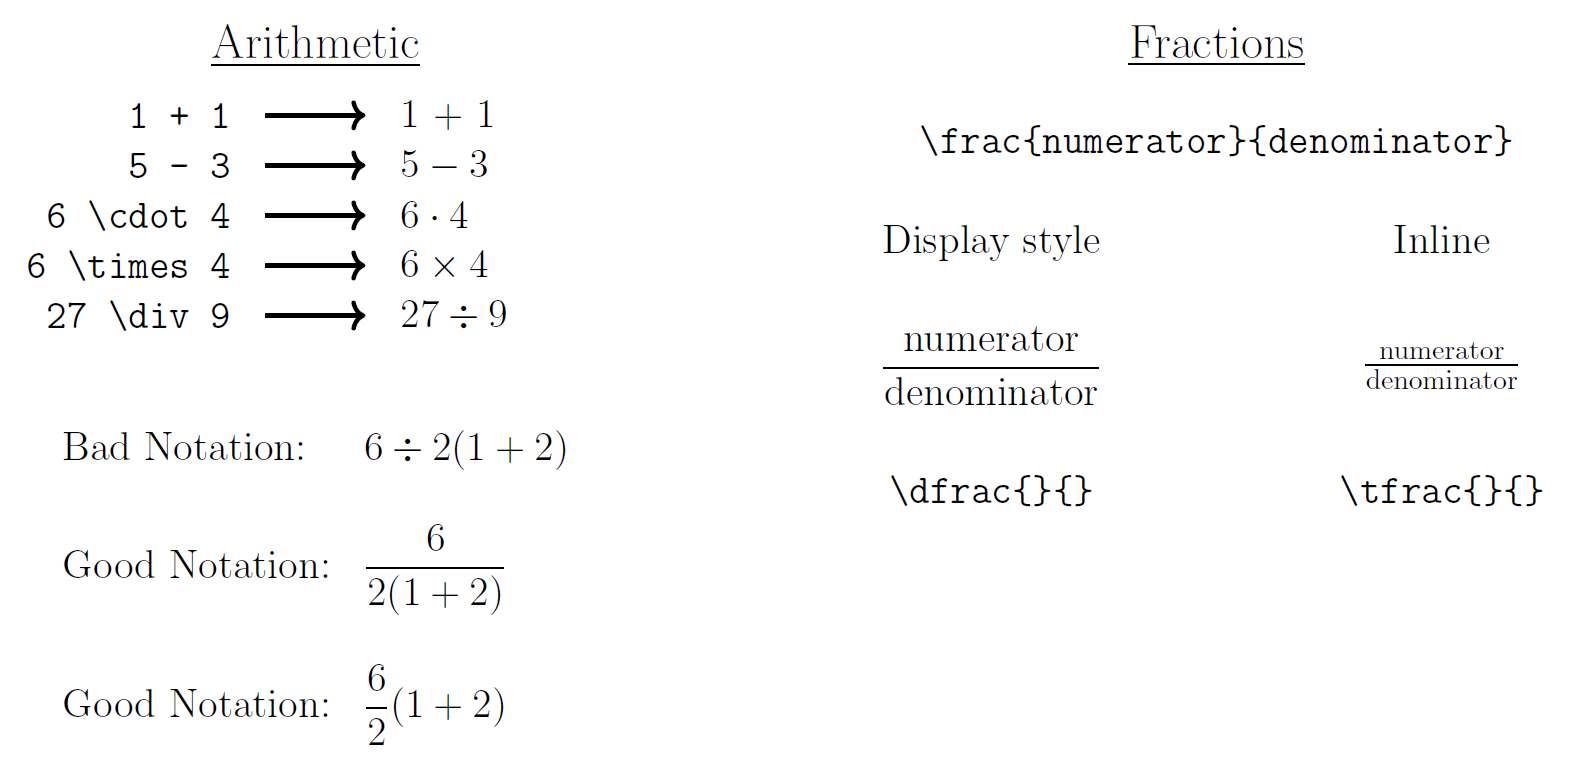
\includegraphics[width=11.5cm]{figs/math4.png}
\end{center}
\end{frame}
%==============================================
\begin{frame}{الصيغ الرياضية و الرموز}
\begin{center}
    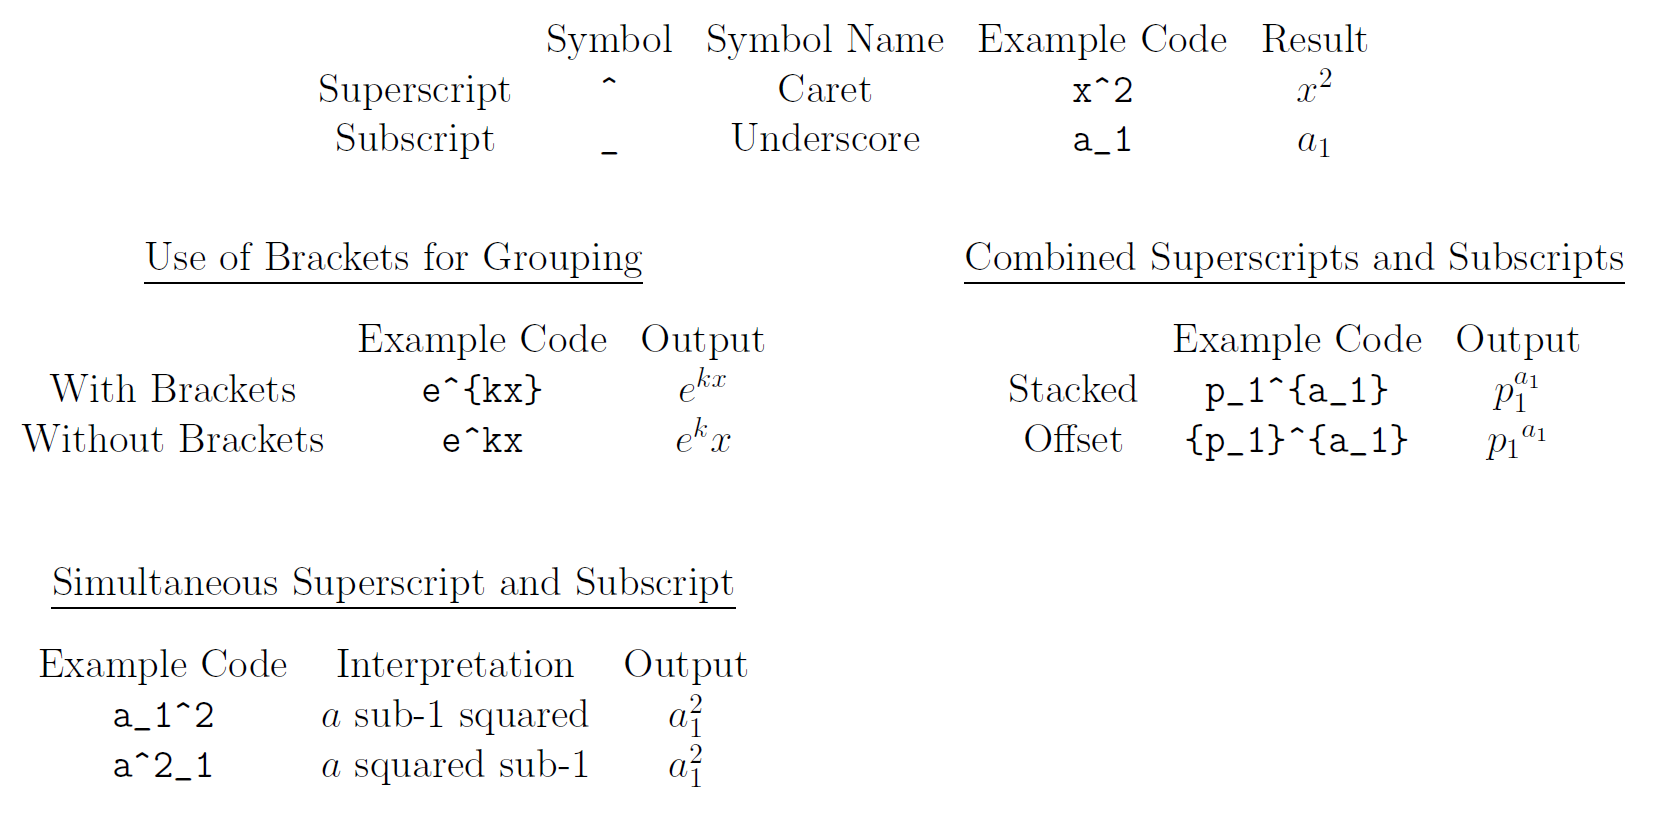
\includegraphics[width=11.5cm]{figs/math6.png}
\end{center}
\end{frame}
%==============================================
\section{ادراج الصور}
\begin{frame}{ادراج الصور}
 %\rtx{https://www1.cmc.edu/pages/faculty/aaksoy/latex/latexthree.html}
\bc
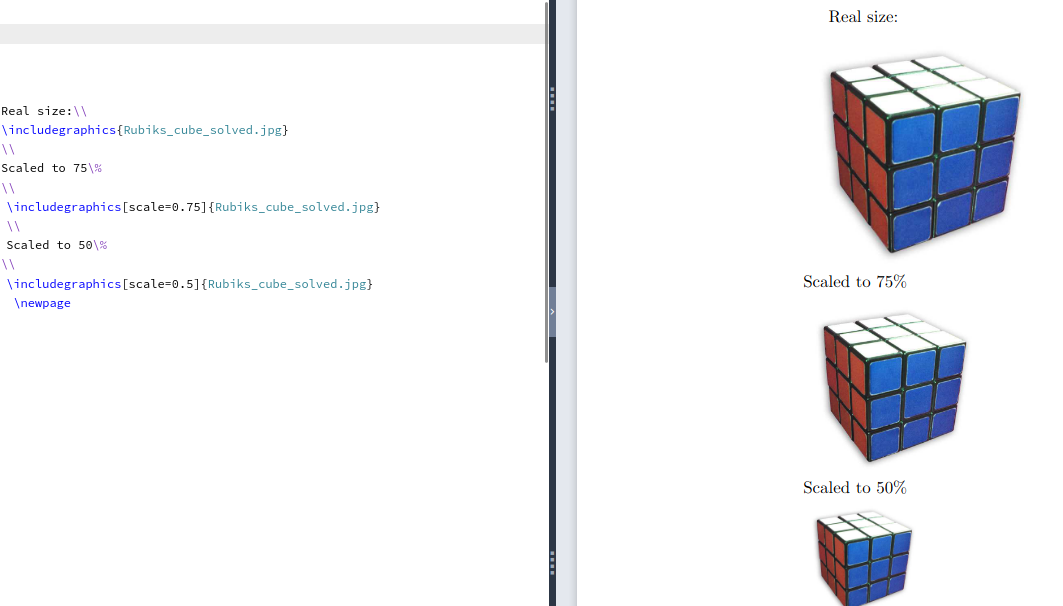
\includegraphics[scale=0.3]{figs/pics1.png}
\ec
\end{frame}

%==============================================
 \begin{frame}{ادراج الصور}
 %\rtx{https://www1.cmc.edu/pages/faculty/aaksoy/latex/latexthree.html}
\bc
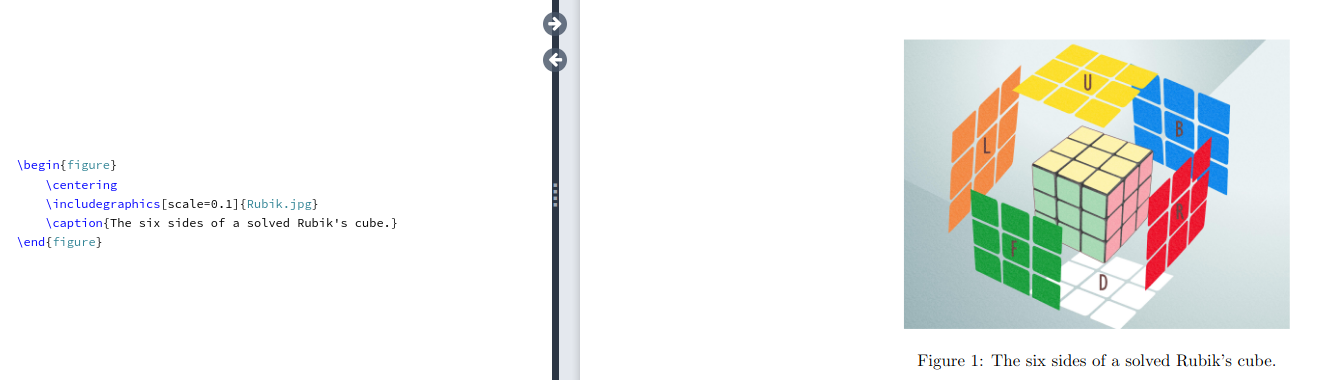
\includegraphics[scale=0.25]{figs/pics2.png}
\ec
\end{frame}
%==============================================
\begin{frame}{روابط مفيدة}
\begin{itemize}\RTListe
    \item\href{https://www.overleaf.com/learn/latex/Tutorials}{تيتوريالات و تمارين  على الموقع الرسمي  ل Overleaf}
    \vspace{0.5cm}
\item \href{https://en.wikipedia.org/wiki/List_of_mathematical_symbols_by_subject}{قائمة الرموز الرياضية حسب الموضوع}
\vspace{0.5cm}
\item \href{https://tex.stackexchange.com/}{موقع أسئلة وأجوبة لمستخدمي \TeX{} و \LaTeX{} }
\vspace{0.5cm}
\item \href{https://www.latex-project.org/help/books/}{كتب مفيدة}
\end{itemize}
\end{frame}

\end{document}